\section{Datengrundlage}

Der Datensatz umfasst 1150 Zeilen mit acht Merkmalen (Alter, Bildungsstufe,
Beschaeftigungsjahre, Wohnjahre, Einkommen, Schulden-Einkommens-Quote,
Kreditkartenschuld, sonstige Schulden) und der Zielvariable \texttt{default}.

\textbf{Nur 700 Zeilen tragen ein Label.} Die uebrigen 450 sind ein Block
ohne Zielvariable; sie enthalten ausserdem nur 150 verschiedene
Merkmalsmuster, jedes dreifach wiederholt. Fuer ueberwachtes Lernen sind sie
unbrauchbar und bleiben aussen vor -- sie dienen hoechstens dem Anwenden eines
fertigen Modells.

Von den 700 gelabelten Kreditnehmern sind \textbf{183
ausgefallen (26,1~\%)} -- ein moderat ungleicher
Datensatz, kein Extremfall.

\begin{figure}[H]
  \centering
  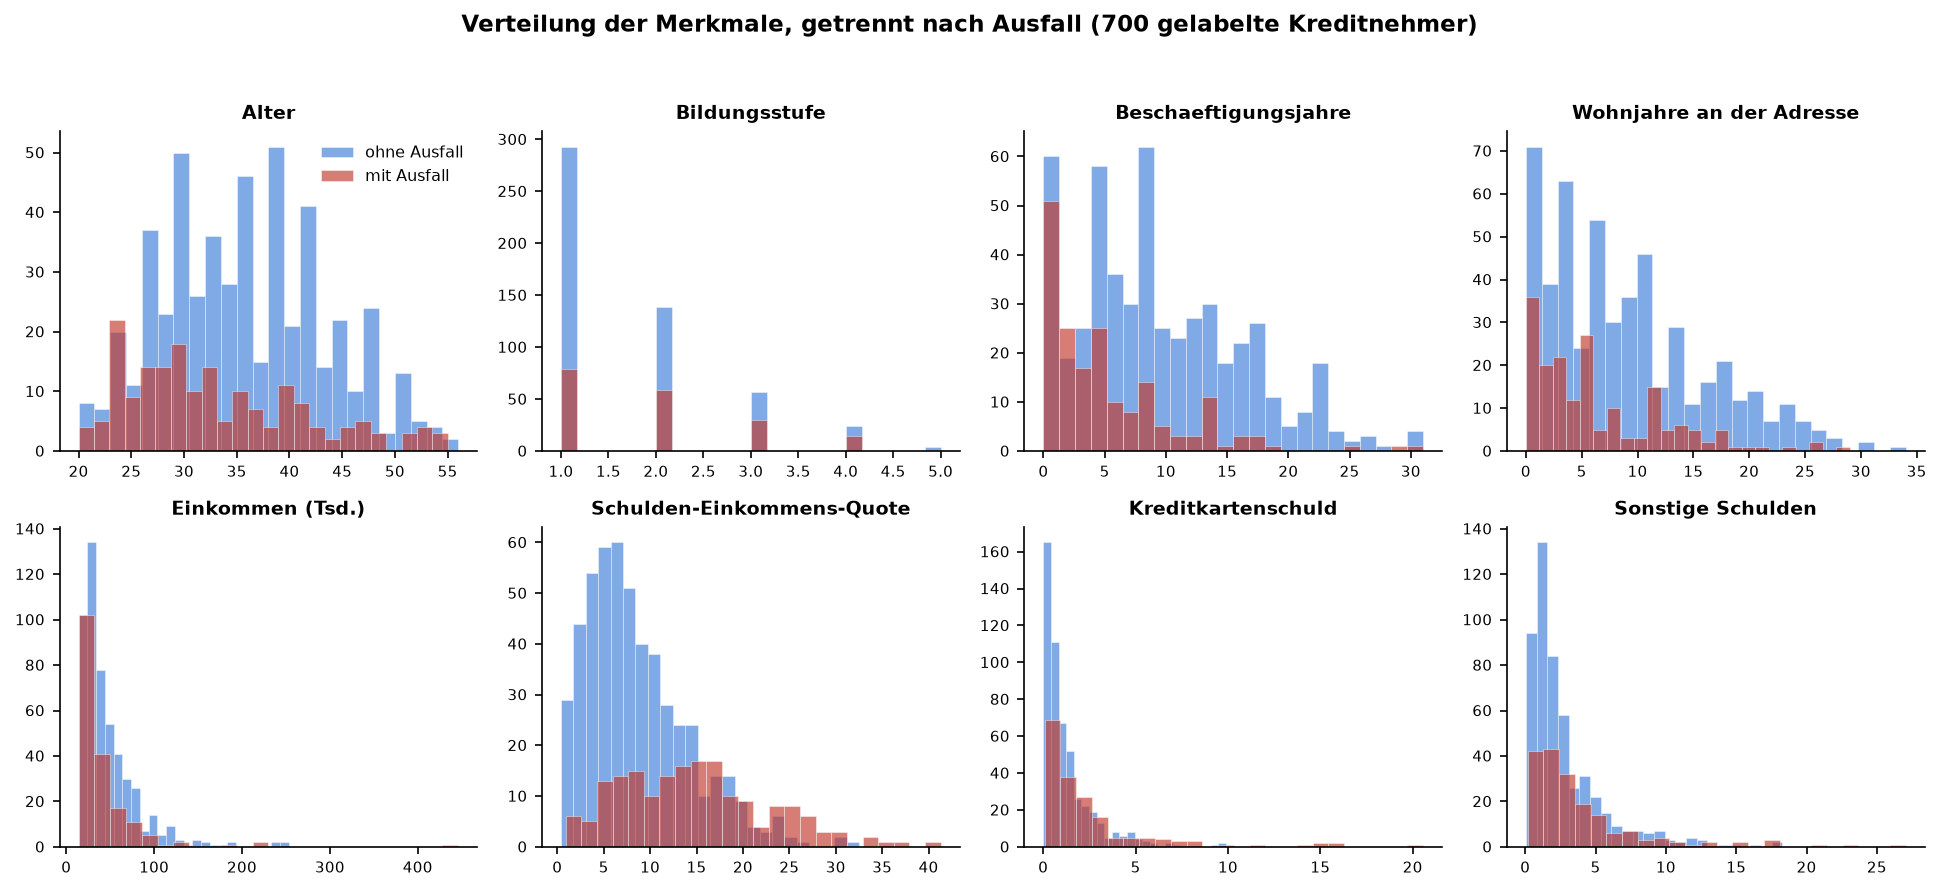
\includegraphics[width=0.90\linewidth]{01_verteilungen.png}
  \caption{Verteilung der Merkmale, getrennt nach Ausfall. Bei der Schulden-Einkommens-Quote und der Kreditkartenschuld liegen die Ausfaller sichtbar rechts, bei den Beschaeftigungs- und Wohnjahren links.}
\end{figure}


\begin{figure}[H]
  \centering
  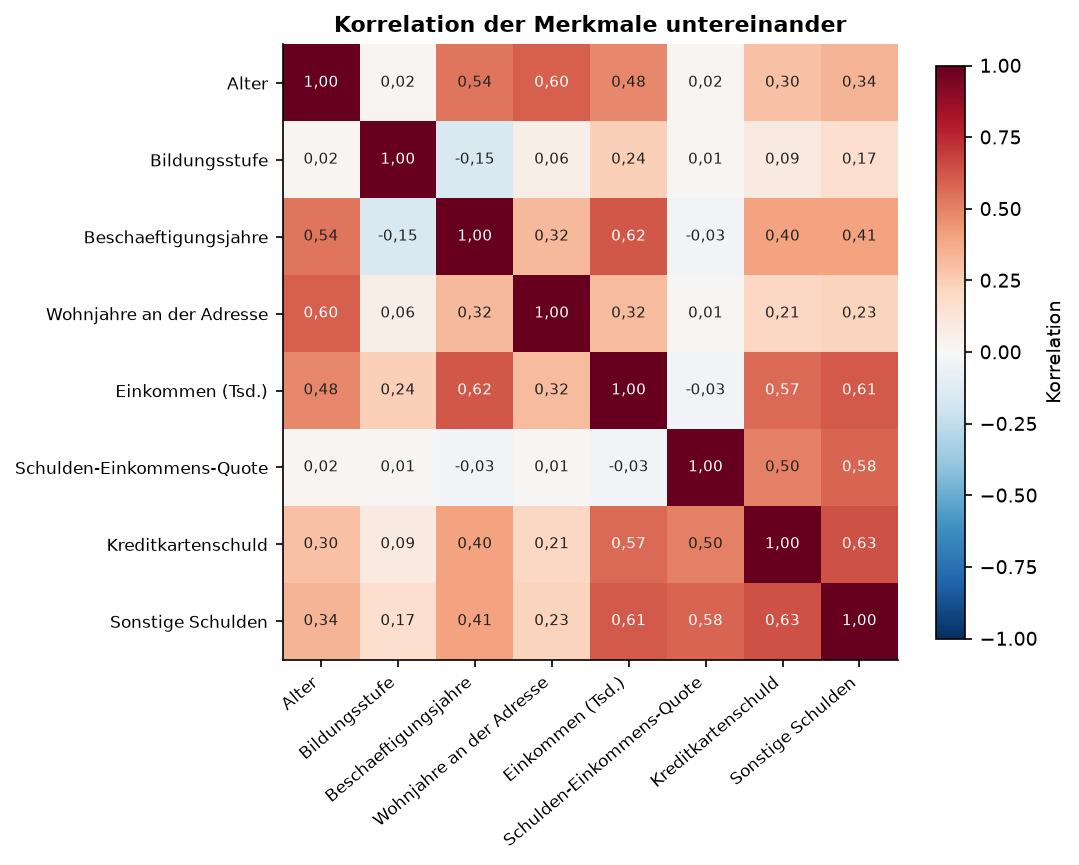
\includegraphics[width=0.90\linewidth]{03_korrelation.png}
  \caption{Korrelation der Merkmale untereinander. Es gibt keine Redundanz, die eine Merkmalsauswahl erzwingen wuerde.}
\end{figure}


\subsection{Was die Merkmale einzeln leisten}

Die Trennschaerfe eines Merkmals allein (AUC; 0,5 bedeutet kein Zusammenhang,
Werte unter 0,5 einen Zusammenhang in die andere Richtung):

\begin{table}[H]
  \centering
  \small
  \begin{tabular}{lr}
    \toprule
    Merkmal & AUC allein \\
    \midrule
    Schulden-Einkommens-Quote & 0,735 \\
    Beschaeftigungsjahre & 0,295 \\
    Kreditkartenschuld & 0,636 \\
    Wohnjahre an der Adresse & 0,389 \\
    Alter & 0,397 \\
    Einkommen (Tsd.) & 0,400 \\
    Sonstige Schulden & 0,587 \\
    Bildungsstufe & 0,574 \\
    \bottomrule
  \end{tabular}
\end{table}


Die \textbf{Schulden-Einkommens-Quote} trennt am besten, gefolgt von der
Kreditkartenschuld. Die Beschaeftigungsjahre wirken in die andere Richtung:
Je laenger jemand beschaeftigt ist, desto geringer das Risiko.

\begin{figure}[H]
  \centering
  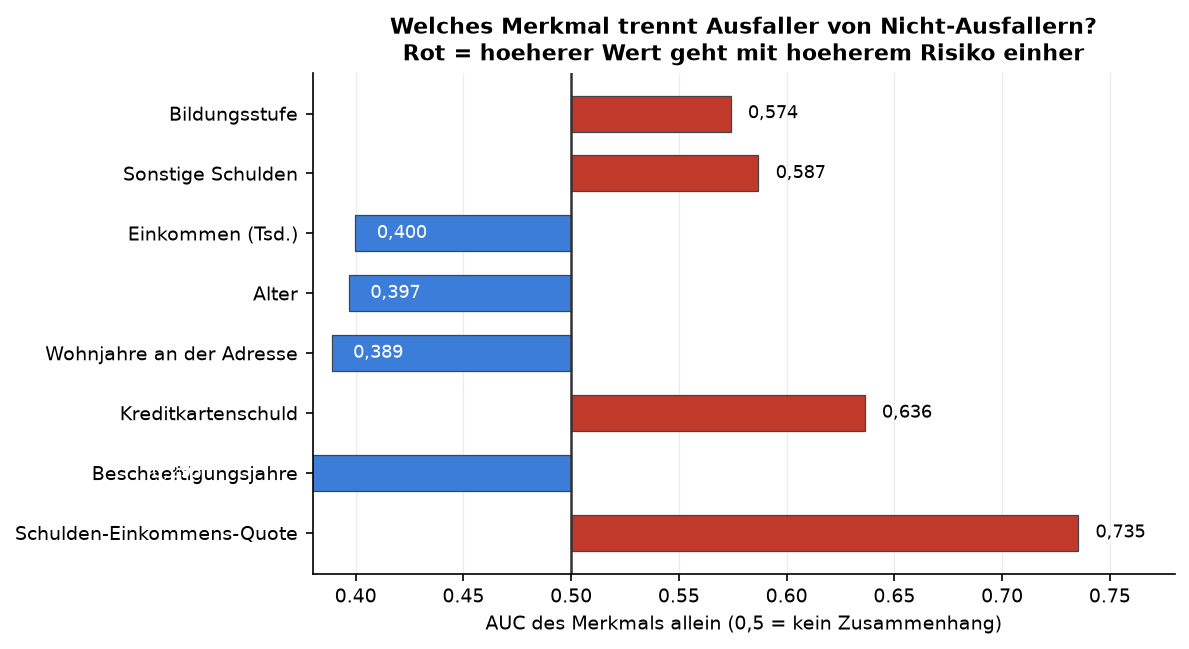
\includegraphics[width=0.90\linewidth]{02_trennschaerfe_einzelmerkmale.png}
  \caption{Trennschaerfe jedes Merkmals allein. Werte ueber 0,5: Ein hoeherer Wert geht mit hoeherem Risiko einher. Werte darunter: mit geringerem.}
\end{figure}


\subsection{Ein scheinbarer Widerspruch, der keiner ist}

Die Ausfallquote steigt mit der Bildungsstufe. Das sieht nach einem starken
Effekt aus, ist aber \textbf{nicht belastbar}:

\begin{table}[H]
  \centering
  \small
  \begin{tabular}{lrrr}
    \toprule
    Bildungsstufe & n & Ausfallquote & KI95 \\
    \midrule
    Stufe 1 & 372 & 21,2 \% & [17,4; 25,7] \\
    Stufe 2 & 198 & 29,8 \% & [23,9; 36,5] \\
    Stufe 3 & 87 & 34,5 \% & [25,3; 44,9] \\
    Stufe 4 & 38 & 36,8 \% & [23,4; 52,7] \\
    Stufe 5 & 5 & 20,0 \% & [3,6; 62,4] \\
    \bottomrule
  \end{tabular}
\end{table}


Die Konfidenzintervalle ueberlappen breit, die oberste Stufe hat nur fuenf
Beobachtungen, und die Korrelation zwischen Bildungsstufe und
Schulden-Einkommens-Quote betraegt 0,009 --
praktisch null. Der Effekt darf nicht als Befund verkauft werden.

\begin{figure}[H]
  \centering
  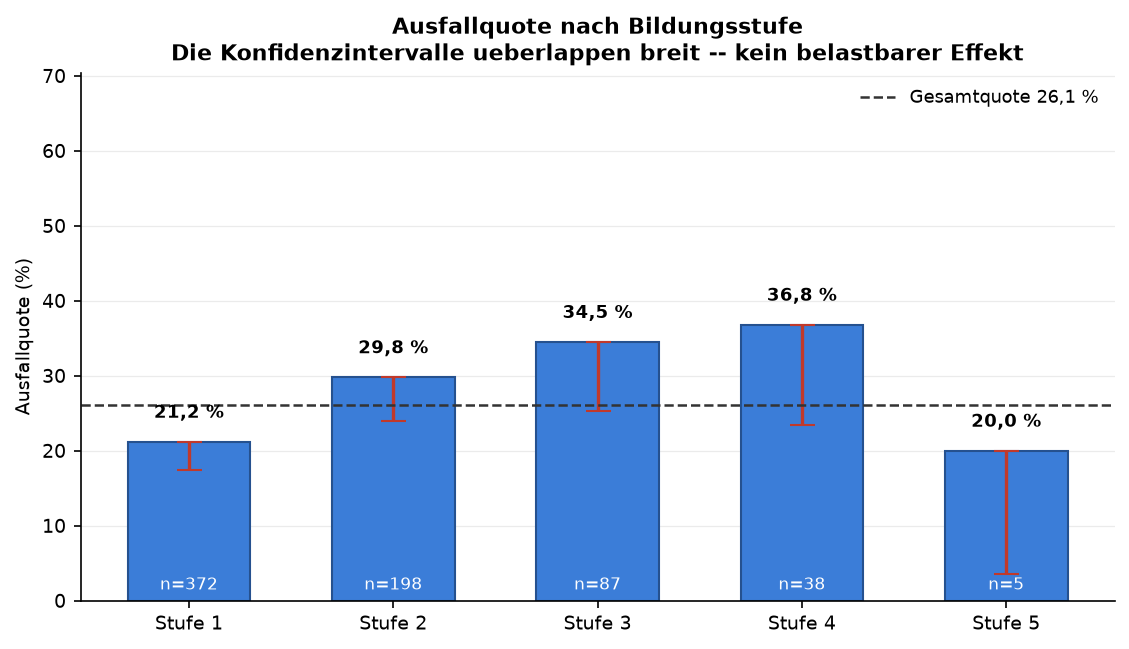
\includegraphics[width=0.90\linewidth]{04_ausfallquote_bildung.png}
  \caption{Ausfallquote je Bildungsstufe mit 95-Prozent-Konfidenzintervall. Der optische Anstieg haelt der Unsicherheit nicht stand.}
\end{figure}

